%%%%%%%%%%%%%%%%%%%%%%%%%%%%%%%%%%%%%%%%%
%% Discussion section
\section{Discussion}

The results show that the recent stagnation in state funding for higher education has affected the composition of faculty within public universities, away from tenure-track and tenured professors towards contingent lecturers.
At the same time, there are little discernible effects on individual professors hired in the years 2011-2021 at Illinois public universities.
The rate that faculty leave their university, and their rate of promotion between positions, are unaffected by the university revenues, so this leaves one primary channel to explain changes in faculty composition: hiring.

The number of professors at a university changes between academic years: professors leave an institution (retiring, hired elsewhere, etc.), while others join (they are newly hired, end a sabbatical, etc.).
Section~\ref{sec:results-indiv} shows that most of these channels are unaffected, implying that falls in hiring for tenured-track and tenured faculty must explain most of the substitution towards lecturers and away from tenured professors.
Notably, faculty hiring is suspected to be impacted by changes in university funding; for example, \cite{turner2014impact} documents the wide-spread practice of hiring freezes at universities in response to budget shocks around the 2008 recession.
Similar measures were taken by Illinois public universities in response to their deteriorating finances in the 2010s \citep{furlough2010}.
The University of Illinois did not receive funding from the state of Illinois before the next fiscal year started, so enacted cost-cutting measures to stay fiscally solvent in the interim.
As one such cost-cutting measure, the university system placed a freeze on all hiring for filling state-funded positions and promotions.

The data used so far measure faculty count, so cannot disentangle which channels are most affected by changes in state funding at a public university.
\autoref{fig:hiring-correlation.png} uses data on the total faculty hired at US public universities over 2011--2021, provided by \cite{wapman2022quantifying},\footnote{
    \cite{wapman2022quantifying} provided an aggregated sample of their data as open-source, making this analysis possible.
} showing a correlation between professor hiring rate and the total state funding per student.
\begin{figure}[h!]
    \centering
    \singlespacing
    \caption{State Funding and Faculty Hired at Public Universities, Total for 2011--2021.}
    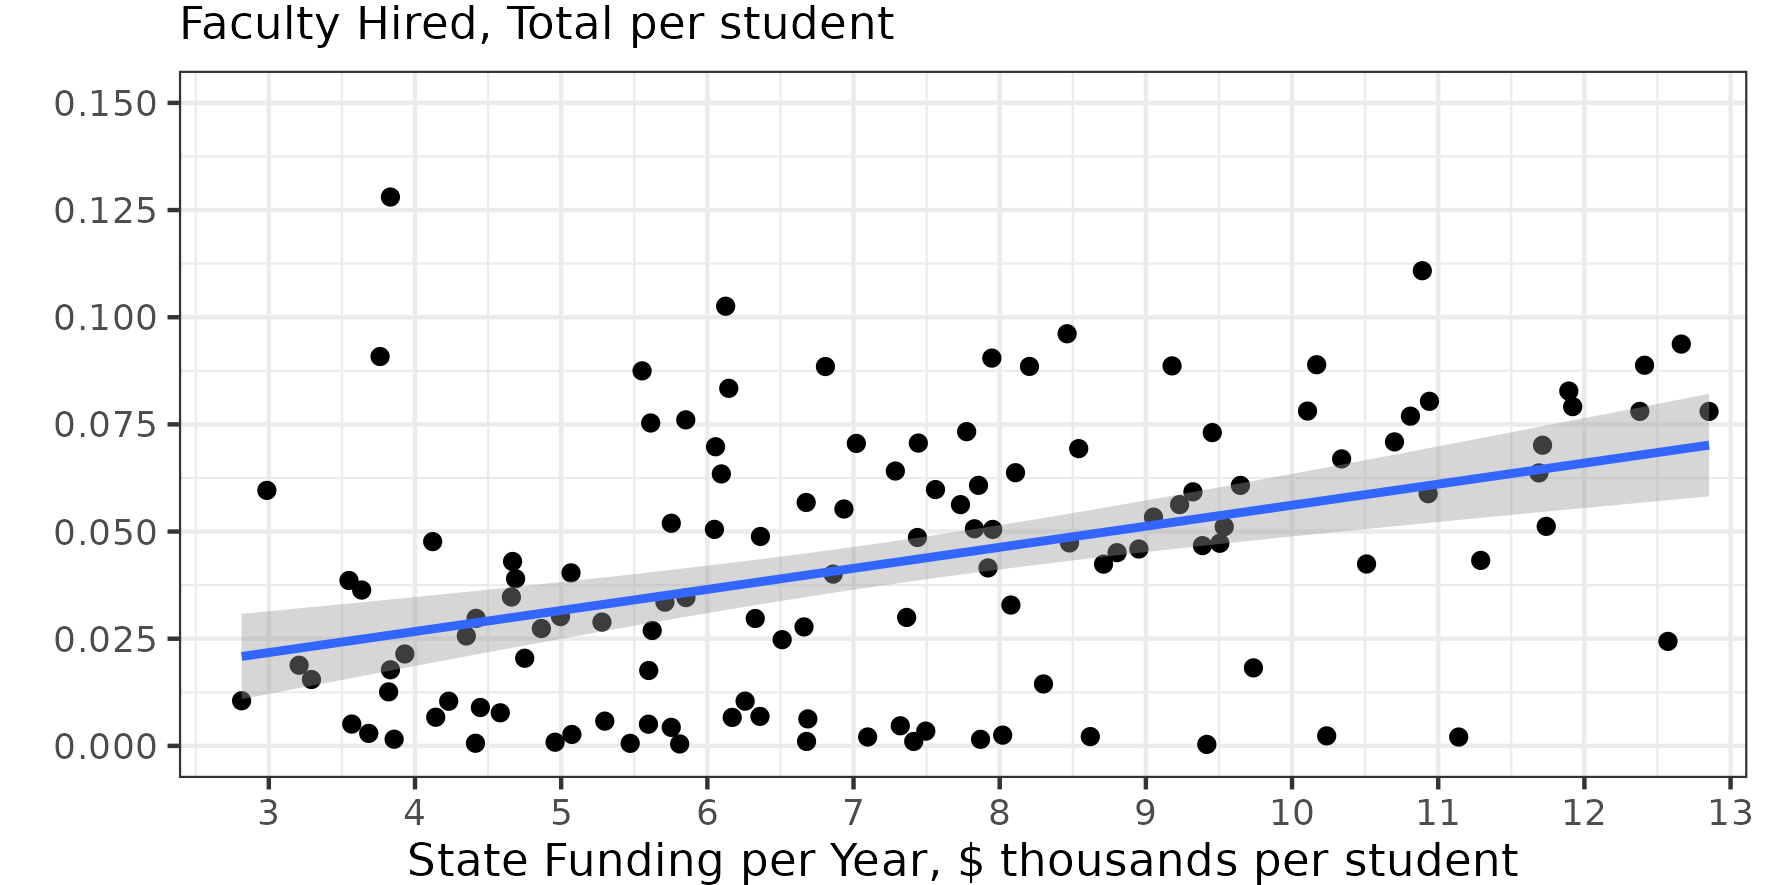
\includegraphics[width=0.8\textwidth]{figures/hiring-correlation.png}
    \label{fig:hiring-correlation.png}
\end{figure}

Universities with more state funding (for the entire decade) hired more professors (\autoref{fig:hiring-correlation.png}).
Similarly, the funding shock IV model shows that a decrease of $-10$\% in state funding leads to $-13$\% fewer faculty hires per student across the decade 2011--2021 (see \autoref{tab:hiring-shock-reg} for full regression model results).\footnote{
    These results were produced by integrating the total count of faculty hires for 2010--2021 for the top-ranked 180 US universities with a sum of the funding variables, and then estimating the models specified in \autoref{sec:iv-model-uni}.
    There were no observable differences in the hiring rate of male vs female faculty.
    See \autoref{sec:appendix-hiring} for further details.
}
It is clear that public universities' hiring is negatively impacted by falls in state funding, even using this highly aggregated count of professor hiring across an entire decade.
While this analysis strengthens the case negative effects on hiring plays, it is crude for measuring exact magnitudes for the effect on faculty hiring.
I leave it to further research to delve deeper into the magnitudes that hiring plays as the primary causal mediator for the effects of falls in state funding on faculty composition at public universities.
